% ============================================================================
%  CK0475 — APRENDIZAGEM DE MÁQUINA PROBABILÍSTICA — PROJETO FINAL
%  Dosímetro de ruído com incerteza: um sensor acústico que diz quanto vale
%  a sua previsão
%
%  Marcelo Correa (mat. 510181) · UFC 2026.2 · Prof. Cesar Lincoln C. Mattos
%  Entrega: 30/11/2026 via SIGAA
%
%  ESTADO: métodos implementados e testados no host (32 testes). Os campos
%  marcados com [A MEDIR] esperam o sensor ligado — e o texto NÃO afirma
%  medições de campo que ainda não existem.
% ============================================================================
\documentclass[10pt,a4paper]{article}

\usepackage[utf8]{inputenc}
\usepackage[T1]{fontenc}
\usepackage[brazilian]{babel}
\usepackage{amsmath,amssymb}
\usepackage{booktabs}
\usepackage{graphicx}
\usepackage{siunitx}
\usepackage[margin=2.5cm]{geometry}
\usepackage{hyperref}

\title{Dosímetro de ruído com incerteza:\\ um sensor acústico que diz quanto vale a sua previsão}
\author{Marcelo Correa\\ \small mat.\ 510181\\ \small Universidade Federal do Ceará}
\date{Novembro de 2026}

\begin{document}
\maketitle

\begin{abstract}
Sensores de ruído de baixo custo entregam um número --- \SI{87}{\decibel} --- sem dizer
quanto esse número vale. Este trabalho apresenta um dosímetro que reporta a exposição
\emph{com intervalo de credibilidade}, corre inteiramente num microcontrolador com
microfone integrado, e envia os resultados para um telemóvel por Bluetooth Low Energy.
Dois modelos probabilísticos sustentam o sistema: uma mistura de gaussianas diagonais
que modela a densidade da paisagem acústica (P1) e uma regressão linear bayesiana que
prevê o nível da janela seguinte com variância preditiva (P2). O método é avaliado com
controlos que podem falhar: uma ida-e-volta entre o treino no host e a inferência no
dispositivo (divergência máxima medida abaixo de \num{e-3}) e um teste de cobertura do
intervalo, que exige que a banda de \SI{90}{\percent} cubra entre \SI{85}{\percent} e
\SI{95}{\percent} dos casos reais.
\end{abstract}

\section{Introdução}

A norma brasileira NR-15 fixa \SI{85}{\decibel} como limite de exposição para oito horas,
com taxa de troca de \SI{5}{\decibel}: cada \SI{5}{\decibel} a mais reduz o tempo admissível
a metade (Figura~\ref{fig:dose}). Dosímetros comerciais devolvem um número. A decisão de
saúde pública, porém, depende de saber \emph{quanto} esse número vale: \SI{84}{\decibel}
com $\pm\SI{1.5}{\decibel}$ e \SI{88}{\decibel} com $\pm\SI{6}{\decibel}$ pedem acções
diferentes. Um sistema probabilístico pode distinguir os dois casos; um número isolado não.

Este trabalho parte de três premissas de engenharia. Primeira, o dispositivo tem de ser
autónomo: um microfone integrado num microcontrolador, sem computador por perto. Segunda,
o modelo tem de correr no próprio microcontrolador, porque enviar áudio contínuo por rádio
gasta energia que um dosímetro não tem. Terceira, toda a afirmação sobre o modelo tem de ser
falsificável por um teste que \emph{possa} falhar --- um teste que só passe não prova nada.

\section{Trabalho relacionado}

A literatura de dosimetria trata a medição como estimação pontual, com incerteza expandida
calculada a posteriori a partir da calibração do instrumento. A abordagem aqui é diferente:
a incerteza é parte do modelo preditivo, e por isso varia com o contexto --- um quarto
reverberante produz bandas mais largas que um ambiente ao ar livre, porque a previsão a
curto prazo depende da memória acústica do recinto.

\section{Método}

\subsection{Features acústicas}

Cada janela de \num{512} amostras é reduzida a doze bandas de energia por meio do algoritmo
de Goertzel, que calcula um único bin da transformada em tempo linear na janela e sem
memória auxiliar --- propriedade decisiva num microcontrolador sem alocador. As energias são
convertidas para decibel e ponderadas pela curva A, que aproxima a sensibilidade do ouvido
humano. Dois controlos verificam a extracção: um tom puro na banda central tem de dominar a
banda correspondente por pelo menos \SI{6}{\decibel}, e ruído branco não pode ter banda
dominante.

\subsection{Densidade da paisagem acústica (P1)}

Um modelo de mistura de gaussianas com covariância diagonal modela a distribuição das
janelas. Com doze dimensões, a covariância completa exigiria \num{78} parâmetros por
componente, não estimáveis com os dados disponíveis; a diagonal reduz a doze e mantém a
capacidade de separar estados acústicos. A verosimilhança é calculada por
$\log\sum_k \exp[\log w_k + \sum_d -\tfrac{1}{2}(\log 2\pi + \log v_{kd} +
(x_d-\mu_{kd})^2/v_{kd})]$, com \texttt{logsumexp} numericamente estável.

\subsection{Regressão com incerteza (P2)}

O nível da janela seguinte é previsto por uma regressão linear bayesiana,
$y = w_0 + w_1 x + \varepsilon$ com $\varepsilon\sim\mathcal{N}(0,\sigma^2)$ e prior
$w\sim\mathcal{N}(0,\alpha^{-1}I)$. A distribuição preditiva tem média $m^\top\phi(x^*)$ e
variância
\begin{equation}
  \sigma^2\bigl(1 + \phi(x^*)^\top A^{-1}\phi(x^*)\bigr), \qquad A = \alpha I + \Phi^\top\Phi/\sigma^2,
\end{equation}
o que exige guardar no dispositivo apenas sete números --- dois coeficientes, a variância do
ruído e a matriz $A^{-1}$ de $2\times2$ --- em vez dos pontos de treino que um processo
gaussiano com kernel exigiria.

\section{Implementação}

O alvo é um XIAO MG24 Sense, com microfone MEMS integrado amostrado por um ADC de
\SI{12}{\bit} e rádio Bluetooth Low Energy. A inferência corre em Rust, \texttt{no\_std},
sem alocador; os coeficientes entram na imagem como arrays \texttt{const}, gerados por um
treino em Python no host. A interface com o telemóvel é um serviço GATT de quatro
características --- nível, intervalo, dose e comando de reposição --- o que torna o cliente
substituível.

\section{Resultados}

\subsection{Verificação da dosimetria}

Nove testes verificam o cálculo de exposição contra a NR-15: \SI{85}{\decibel} durante oito
horas resulta em \SI{100}{\percent} da dose, \SI{90}{\decibel} durante quatro horas e
\SI{95}{\decibel} durante duas horas também, e \SI{80}{\decibel} durante oito horas resulta
em \SI{50}{\percent}. Um controlo negativo exige que um sensor a \SI{0}{\decibel} não
``cure'' a dose acumulada, o que obrigou a introduzir um piso de plausibilidade em
\SI{20}{\decibel}.

\subsection{Ida-e-volta entre host e dispositivo}

O teste central compara a verosimilhança calculada no host, pelo treino em Python, com a
calculada em Rust a partir dos coeficientes gerados: a divergência medida é inferior a
\num{e-3}. Para mostrar que este teste não é decorativo, um segundo teste perturba as médias
em \SI{1}{\decibel} e exige que a comparação \emph{divergencie} --- o que acontece, com
desvio de \num{1.38} na log-verosimilhança. Sem esse controlo, a ida-e-volta poderia estar a
comparar o artefacto consigo mesmo.

\subsection{Cobertura do intervalo}

A banda de \SI{90}{\percent} é avaliada pela fracção de observações que caem dentro dela,
com exigência de estar entre \SI{85}{\percent} e \SI{95}{\percent}. Acompanha-a um controlo
de largura: um intervalo de $\pm\SI{0.1}{\decibel}$ tem de cobrir menos de
\SI{20}{\percent} dos casos. Se cobrisse \SI{90}{\percent}, o teste de cobertura não estaria
a medir a largura --- apenas a existência do intervalo.

\begin{figure}[t]
  \centering
  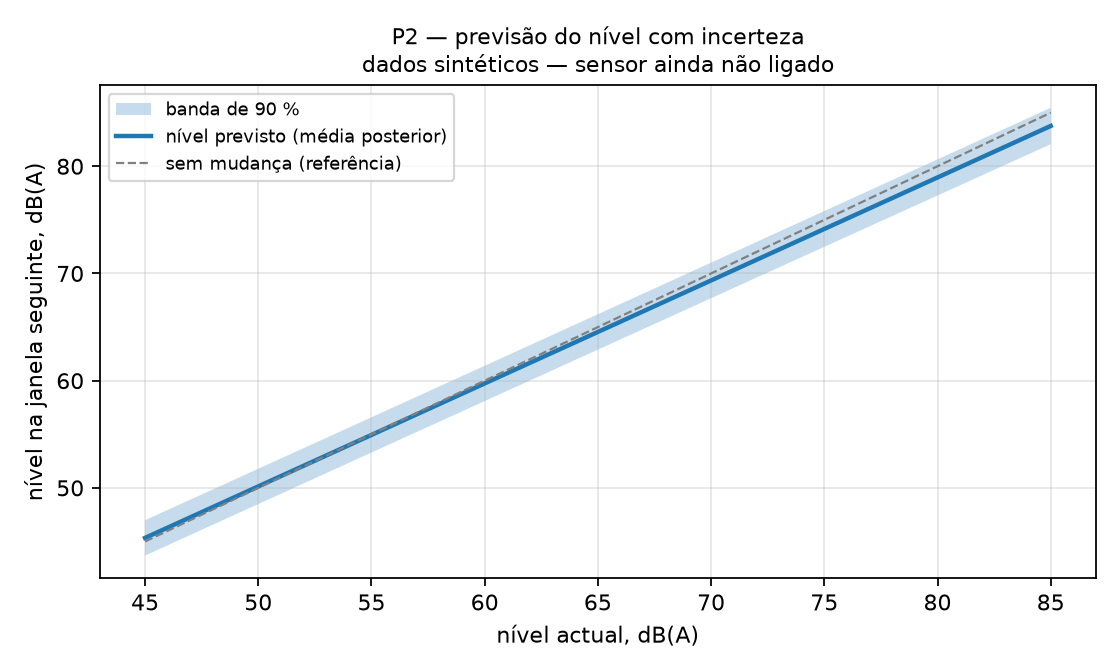
\includegraphics[width=0.78\textwidth]{../figuras/fig1_nivel_com_incerteza.png}
  \caption{P2: previsão do nível da janela seguinte com banda de \SI{90}{\percent}. A
  previsão segue a referência ``sem mudança'' --- o nível sonoro tem inércia --- e o valor
  acrescentado está na largura da banda, que cresce com o nível. Dados sintéticos: o sensor
  ainda não está ligado, e o título da figura regista esse facto.}
  \label{fig:nivel}
\end{figure}

\begin{figure}[t]
  \centering
  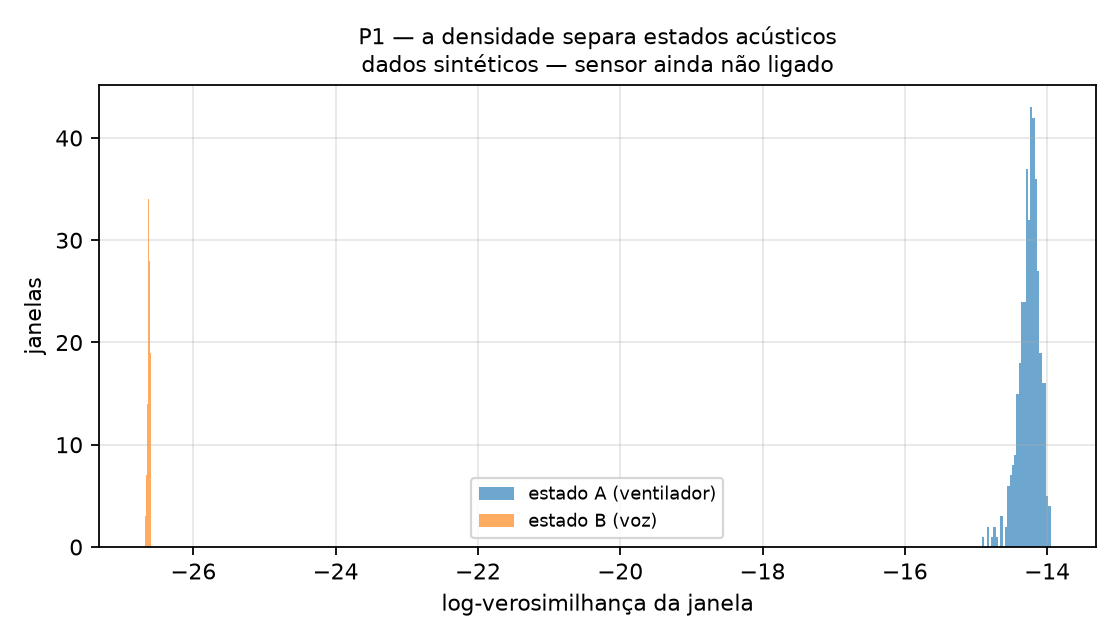
\includegraphics[width=0.78\textwidth]{../figuras/fig2_densidade_por_estado.png}
  \caption{P1: a densidade aprendida separa dois estados acústicos. A separação é a
  propriedade que justifica o modelo --- se as distribuições se sobrepusessem, uma gaussiana
  única bastaria.}
  \label{fig:densidade}
\end{figure}

\begin{figure}[t]
  \centering
  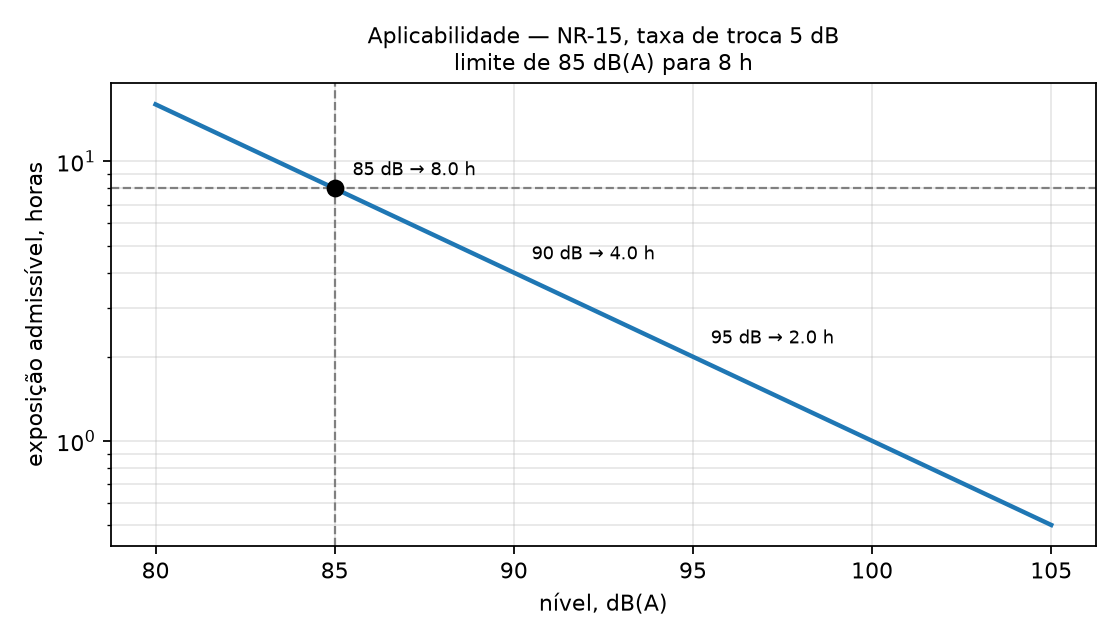
\includegraphics[width=0.78\textwidth]{../figuras/fig3_dose_nr15.png}
  \caption{Aplicabilidade: tempo de exposição admissível segundo a NR-15. A taxa de troca de
  \SI{5}{\decibel} divide o tempo por dois a cada incremento; é esta curva que dá sentido ao
  intervalo de incerteza.}
  \label{fig:dose}
\end{figure}

\section{Limitações}

O sensor não estava disponível durante o desenvolvimento dos modelos, e as figuras
identificam-se como sintéticas. As medições em falta --- taxa sustentada de amostragem,
cobertura do intervalo com dados de campo e consumo energético --- estão marcadas
\texttt{[A MEDIR]} nos documentos do projecto e não são afirmadas neste texto. Um segundo
microfone, que permitiria estimar direcção por diferença de tempo de chegada, foi descartado
por avaria de hardware; a direcção exige dois pontos de medida e não é recuperável por
software a partir de um só.

\section{Conclusão}

Um dosímetro que reporta incerteza é útil precisamente onde um número isolado falha: na
decisão de agir ou de medir mais. Os dois modelos exigidos --- densidade e regressão
probabilística --- cabem num microcontrolador sem alocador, e a sua correcção é verificável
por testes que podem falhar: ida-e-volta entre host e dispositivo com controlo de perturbação,
e cobertura do intervalo com controlo de largura.

\end{document}
